\section{Materiales y métodos}
\label{sec:metodos}

\subsection{Base de datos y alcance}
\label{sec:base}
% Módulo: M0

Se usa la base PH2 \parencite{mendonca2013}, del Hospital Pedro Hispano (Portugal). Contiene 200 imágenes dermatoscópicas RGB de 8 bits por canal, adquiridas con el mismo equipo y en condiciones uniformes: 80 nevos comunes, 80 nevos atípicos y 40 melanomas. El tamaño de las imágenes no es fijo: hay 24 tamaños distintos, los más frecuentes de $767\times576$ y $768\times576$ píxeles, por lo que ninguna etapa del algoritmo supone un tamaño determinado. La lesión ocupa entre el 3\,\% y el 98\,\% de la imagen (mediana 23\,\%), y en 50 imágenes toca el borde, es decir, no se ve completa. Cada imagen viene con la máscara de la lesión dibujada a mano y con la evaluación de un dermatólogo: diagnóstico clínico, asimetría (0, 1 o 2 ejes), colores presentes (de los seis de la regla) y presencia de red de pigmento (típica o atípica), puntos y glóbulos, estrías, áreas de regresión y velo azul-blanquecino. En 27 imágenes se incluyen además máscaras de las regiones de cada color. Eso permite validar el algoritmo paso a paso: la segmentación contra la máscara, A y C contra el dermatólogo, la textura contra las estructuras anotadas y la clasificación contra el diagnóstico.

Se trabaja con las 200 imágenes. Se considera \emph{sospechosa} toda lesión con diagnóstico de nevo atípico o melanoma (120 imágenes) y \emph{no sospechosa} a los nevos comunes (80), lo que responde a la pregunta del anteproyecto: distinguir las lesiones que ameritan control de los lunares comunes. El recorte de alcance sugerido en la devolución se aplica sobre los objetivos: la evaluación completa del algoritmo sobre imágenes comprimidas queda como objetivo de máxima.

Para el criterio D adaptado se cuenta la cantidad de estructuras presentes según el dermatólogo (0 a 5). La red de pigmento se cuenta sólo cuando es atípica. En la regla original se cuenta su presencia \parencite{nachbar1994}, pero en PH2 todas las lesiones tienen red (típica o atípica), así que su mera presencia no distingue entre lesiones; se usa en cambio la red atípica, que es la que se asocia al melanoma \pendiente{citar}. Con esta definición, la red atípica no aparece en ningún nevo común y sí en 77 de los 80 atípicos y 39 de los 40 melanomas, y el D medio es 0,65 en los nevos comunes, 1,79 en los atípicos y 3,12 en los melanomas.

Las imágenes se dividieron en un conjunto de entrenamiento (70\,\%, 140 imágenes) y uno de prueba (30\,\%, 60 imágenes), estratificados por diagnóstico y con semilla fija para que la partición sea reproducible (tabla~\ref{tab:particion}). Todos los umbrales y parámetros se eligen únicamente con el conjunto de entrenamiento; el de prueba se usa sólo para las métricas finales.

\begin{table}[h]
  \centering\small
  \begin{tabular}{@{}lccc|c@{}}
    \toprule
    Conjunto & Nevo común & Nevo atípico & Melanoma & Total \\
    \midrule
    Entrenamiento & 56 & 56 & 28 & 140 \\
    Prueba        & 24 & 24 & 12 & 60 \\
    \midrule
    Total         & 80 & 80 & 40 & 200 \\
    \bottomrule
  \end{tabular}
  \caption{Cantidad de imágenes por diagnóstico en cada conjunto.}
  \label{tab:particion}
\end{table}

\pendiente{Figura con un ejemplo de cada diagnóstico y el contorno de su máscara (\texttt{m0\_ejemplos}, del cuaderno de M0).}

\subsection{Esquema del algoritmo}
\label{sec:esquema}
\pendiente{Diagrama de bloques: imagen $\rightarrow$ mejoramiento (viñeta, pelos) $\rightarrow$ segmentación $\rightarrow$ criterios A, B, C $\mid$ textura y D $\mid$ zonas y mapas $\rightarrow$ TDS (y TDS extendido) $\rightarrow$ clasificación. Indicar el módulo del repositorio de cada bloque.}

\subsection{Pre-procesamiento}
\label{sec:preprocesamiento}

\subsubsection{Análisis exploratorio y mejoramiento}
% Módulo: M1
\textbf{Análisis exploratorio.} Con las imágenes de entrenamiento se eligió el canal con más contraste entre lesión y piel: en cada imagen se tomaron 2000 píxeles de la lesión (máscara de PH2) y 2000 de piel, y se calculó el área bajo la curva ROC (AUC) de separarlos con un umbral sobre cada canal (R, G, B, H, S, V, L de Lab y gris). También se estimaron valores de referencia en HSV de cada color a partir de las máscaras de color que PH2 incluye en 27 imágenes.

\textbf{Viñeteo.} Las esquinas oscuras que deja la lente circular se excluyen con una máscara de píxeles válidos. No se usó un umbral fijo de brillo, porque el brillo de las esquinas varía mucho entre imágenes ($V$ entre 0,13 y 0,77) y un umbral que las capture a todas captura también zonas oscuras de 124 de las 140 lesiones de entrenamiento; además, en 50 imágenes la lesión toca el borde. En cambio se aprovecha que la viñeta es circular y centrada: se calcula la mediana de $V$ en anillos concéntricos de 4 píxeles y la viñeta empieza en el primer anillo cuya mediana cae por debajo del 60\,\% del anillo más brillante (figura~\ref{fig:vineta}). La mediana no se ve afectada por una lesión que ocupa sólo una parte del anillo. Para lesiones muy grandes, que ocupan anillos completos, se impone que la viñeta no empiece antes del 80\,\% de la semidiagonal de la imagen.

\textbf{Pelos.} Se detectan con un cierre morfológico del gris con elementos estructurantes lineales de 21 píxeles en 12 orientaciones (cada \ang{15}), tomando el máximo de los cierres: se rellena toda zona oscura que mida menos de 21 píxeles en alguna dirección. Los píxeles donde la diferencia entre el cierre y la imagen original (\emph{black-hat}) supera 0,10 son candidatos \parencite{lee1997}. Como la red de pigmento y los glóbulos también son oscuros y finos, sólo se conservan las regiones con forma de pelo: esqueleto de al menos 60 píxeles, ancho medio (área/largo del esqueleto) de a lo sumo 8 píxeles y eje mayor de al menos 80 píxeles. Los píxeles de pelo se reconstruyen por \emph{inpainting} \parencite{telea2004} y el resto de la imagen no se modifica. Para la hipótesis~1 se compara con no quitar los pelos y con un filtro de mediana de $9\times9$ por canal. La tabla~\ref{tab:param-m1} resume los parámetros.

\begin{figure}[h]
  \centering
  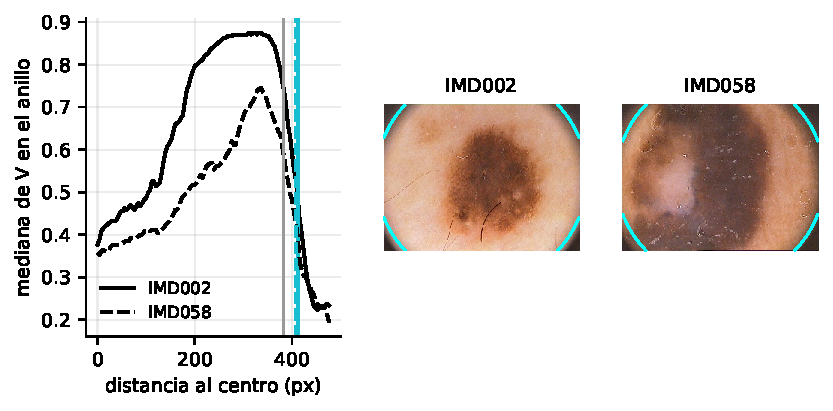
\includegraphics[width=0.85\textwidth]{m1_vineta}
  \caption{Detección del viñeteo. Izquierda: mediana del brillo $V$ en anillos concéntricos para una imagen típica (IMD002) y una con la lesión tocando el borde (IMD058); las líneas verticales marcan el radio detectado. Derecha: límite de la zona válida sobre ambas imágenes.}
  \label{fig:vineta}
\end{figure}

\begin{table}[h]
  \centering\small
  \begin{tabular}{@{}lll@{}}
    \toprule
    Etapa & Parámetro & Valor \\
    \midrule
    Viñeta & Anillo / umbral / radio mínimo & 4 px / 0,6 del máximo / 0,8 semidiagonal \\
    Pelos  & Elemento estructurante & segmento de 21 px, 12 orientaciones \\
           & Umbral del \emph{black-hat} & 0,10 \\
           & Forma: largo / ancho / eje mayor & $\ge 60$ px / $\le 8$ px / $\ge 80$ px \\
           & Reconstrucción & \emph{inpainting} de Telea, radio 5 px \\
    Comparación & Filtro de mediana & $9\times9$ por canal \\
    \bottomrule
  \end{tabular}
  \caption{Parámetros del mejoramiento (módulo M1), elegidos con el conjunto de entrenamiento.}
  \label{tab:param-m1}
\end{table}

\subsubsection{Compresión y descompresión}
% Módulo: M2
\pendiente{Las imágenes se comprimen con JPEG a distintas calidades y se descomprimen; se mide la tasa de compresión, el PSNR (en toda la imagen y dentro de la lesión) y el SSIM \parencite{wang2004}.}

\subsection{Segmentación}
\label{sec:segmentacion}
% Módulo: M3
Se comparan el umbral de Otsu \parencite{otsu1979}, el crecimiento de regiones desde el centro de la imagen, k-means y el modelo de Chan-Vese \parencite{chan2001}. Luego se aplica una apertura para eliminar islas, un cierre para unir los huecos del borde y, con el etiquetado, se conserva la región que contiene el centro. Se elige el método con mayor Dice medio en entrenamiento.
\pendiente{Método elegido y parámetros.}

\subsection{Criterios A, B y C}
\label{sec:abc}
% Módulo: M4
\textbf{Asimetría:} se calculan el centroide y los ejes principales de la máscara, se la refleja sobre cada eje y se mide la fracción de área que no se superpone. Un eje es asimétrico si esa fracción supera un umbral, elegido en entrenamiento para coincidir lo más posible con el dermatólogo, y $A$ es la cantidad de ejes asimétricos. \textbf{Borde:} la lesión se divide en 8 sectores y en cada uno se calcula, con el filtro de Sobel sobre $V$, el gradiente medio sobre el contorno; los sectores con gradiente alto cuentan como borde abrupto. \textbf{Color:} cada píxel se asigna al más cercano de los seis colores de referencia en HSV, y un color está presente si ocupa más de un porcentaje mínimo de la lesión. Se calcula además la circularidad $4\pi\,\text{área}/\text{perímetro}^2$.
\pendiente{Umbrales elegidos y cómo; referencias HSV de los seis colores.}

\subsection{Textura y criterio D adaptado}
\label{sec:textura}
% Módulo: M5
Se calcula la GLCM sobre $V$ dentro de la lesión, promediada en las cuatro direcciones, y sus atributos de energía, entropía, contraste, IDM, correlación, \emph{cluster shade} y \emph{cluster prominence} \parencite{haralick1973}. Como PH2 no anota exactamente las cinco estructuras de la regla, se usa un $D$ adaptado: la cantidad de estructuras que el dermatólogo marcó como presentes. Para estimarlo en una imagen nueva se usa el atributo que más cambia con esa cantidad en entrenamiento, con umbrales que separan los distintos valores de $D$.
\pendiente{Niveles de gris, distancia, atributo elegido y umbrales.}

\subsection{Zonas de la lesión y mapas de características}
\label{sec:zonas}
% Módulo: M6
\pendiente{(Devolución) Definición de centro, periferia e interfases interna y externa (transformada de distancia, anchos); atributos por zona; contrastes entre zonas propuestos como términos del TDS; mapas de características por ventanas. Figura con las zonas sobre una lesión.}

\subsection{Clasificación}
\label{sec:clasificacion}
% Módulo: M7
Una lesión se clasifica como sospechosa si su TDS automático (ec.~\ref{eq:tds}) supera un umbral. Se comparan el umbral clínico (4,75) con el que maximiza la suma de sensibilidad y especificidad en entrenamiento (índice de Youden, \cite{youden1950}). Para la hipótesis 2 se define un TDS extendido sumando al TDS los términos de textura y de zonas elegidos en entrenamiento, estandarizados con la media y el desvío de entrenamiento, y se vuelve a elegir el umbral.
\pendiente{Términos elegidos.}

\subsection{Evaluación}
\label{sec:evaluacion}
Sobre el conjunto de prueba, la segmentación se compara con la máscara de PH2 mediante el coeficiente de Dice. Los criterios A y C se comparan con el dermatólogo mediante el $\kappa$ de Cohen \parencite{cohen1960}; valores entre 0,41 y 0,60 se consideran un acuerdo moderado \parencite{landis1977}. La clasificación se mide con la sensibilidad, la especificidad y el área bajo la curva ROC (AUC). Para H1 se compara, en las imágenes con pelos, el Dice sin quitar los pelos, con mediana y con cierre; para H2, las métricas del TDS y del TDS extendido.
\pendiente{Prueba de significancia (p. ej. bootstrap del AUC o prueba de Wilcoxon para el Dice pareado).}

\subsection{Interfaz gráfica}
\label{sec:interfaz}
% Carpeta: interfaz/
\pendiente{Aplicación en Streamlit (\texttt{streamlit run interfaz/app.py}): captura y descripción breve de su manejo (elegir imagen y métodos; ver máscara de pelos, contorno, colores, zonas, mapa de textura, A, B, C, D, TDS y clasificación).}

\subsection{Código y repositorio}
\label{sec:codigo}
La consigna pide detallar el contenido de cada archivo de Python. El código está en el repositorio \pendiente{link}. Cada módulo tiene un archivo \texttt{.py} con las funciones y un cuaderno \texttt{.ipynb} con las pruebas, figuras y discusión.

\begin{table}[h]
  \centering\footnotesize
  \begin{tabular}{@{}lll@{}}
    \toprule
    Carpeta & Archivo & Contenido \\
    \midrule
    raíz & \texttt{main.py} & Verifica módulos, procesa imágenes y genera resultados \\
    M0 & \texttt{carga\_de\_datos.py} & Lectura de PH2, alcance y partición \\
    M1 & \texttt{mejoramiento.py} & Viñeta y remoción de pelos \\
    M2 & \texttt{compresion.py} & JPEG, tasa de compresión, PSNR y SSIM \\
    M3 & \texttt{segmentacion.py} & Métodos de segmentación, posprocesamiento y Dice \\
    M4 & \texttt{criterios\_abc.py} & Asimetría, borde, colores y circularidad \\
    M5 & \texttt{textura\_criterio\_d.py} & GLCM y criterio D adaptado \\
    M6 & \texttt{zonas\_y\_mapas.py} & Zonas de la lesión y mapas de características \\
    M7 & \texttt{clasificacion\_resultados.py} & TDS, umbrales, métricas y figuras finales \\
    herramientas & \texttt{*.py} & Pegamento, verificación, gráficos y lesiones de prueba \\
    interfaz & \texttt{app.py} & Interfaz gráfica \\
    \bottomrule
  \end{tabular}
  \caption{Archivos de Python del repositorio. Cada módulo M$n$ está en \texttt{modulos/m$n$\_\ldots/}.}
  \label{tab:archivos}
\end{table}
